\overlays{3}{
\begin{slide}{GNU: Gnu's Not Unix}

{\red {\small Si è parlato spesso di GNU\dots Cos'è il "Progetto GNU" ?}}

\onlySlide*{1}{
Bisogna sapere che in origine il mondo dell'informatica era molto
diverso. Quando i computer occupavano ancora intere stanze, tutto il
software circolava liberamente con il solo scopo di progredire nella
tecnologia e nell'informatica. UNIX era il sistema operativo in voga
all'epoca. Nato per fini più pratici che teorici, era distribuito
liberamente.
}

\onlySlide*{2}{
\tiny{
Un giorno, molte aziende cominciarono ad acquistare UNIX,
modificarlo e cambiare la sua licenza così chè esso divenne chiuso, a
pagamento e chi lo usava non poteva avere accesso al suo codice
sorgente, non poteva studiarne il funzionamento, modificarlo qualora ne
avesse bisogno e gli stessi sviluppatori che lo avevano creato non potevano, legati da
contratto, rivelare niente che riguardasse il sistema operativo.

La forte comunità scientifica che si era creata intorno ad UNIX, fatta
di scambio libero del sapere, codice libero, licenze praticamente
assenti, aiuto reciproco e amicizia venne di colpo stroncata.
}}

\onlySlide*{3}{
{\tiny
Un ricercatore, però, si oppose a tutto questo.

Rifiutando contratti favolosi, posti di lavoro eccellenti e paghe
profumate, Richard Matthew Stallman decise che avrebbe creato un suo
sistema operativo.

Un sistema operativo che avrebbe avuto l'obbiettivo principale di essere
\emph{libero}. 

Un sistema operativo che fosse simile ad UNIX, visto che UNIX funzionava
abbastanza bene, ma che non ne fosse una copia pari pari. Così venne GNU: 
}

\center{Gnu's Not Unix}

\begin{tabular}{lcr}

\includegraphics[width=0.25\columnwidth,height=0.30\textheight]{immagini/gnu.eps} &%
&%
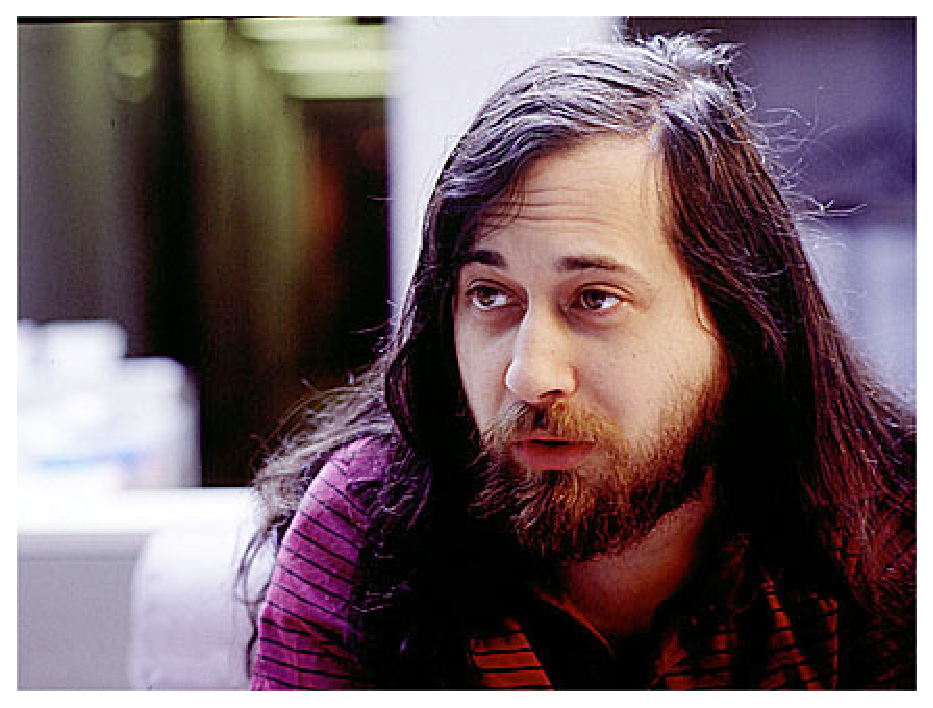
\includegraphics[width=0.25\columnwidth,height=0.30\textheight]{immagini/stallman.eps}%

\end{tabular}



}

\end{slide}}
